\chapter{TBD: Findings and Results}
For now, this chapter is a placeholder for the findings and results. Some were misplaced earlier in the thesis, others need to be written and then woven into the narrative.


%%%% 02 Jul 2021
% Aim to migrate all the findings to the relevant case study.

\section{Findings}
\label{findings-section}

To Discuss:
\begin{itemize}
    \item Findings in the analytics
    \item Results in applying analytics
    \item Flaws in the analytics tools
    \item Results of using flawed analytics tools
    \item Software created to enable aspects of the research
    \item Results of the software we created for the research
\end{itemize}

The application of mobile analytics has enabled each of the development teams who participated in the research to materially improve their measured reliability. 

For the first case study the reliability was improved approximately 12x for the main Kiwix Android application by applying the approach identified in this research. 
During the initial improvement stages the reliability of the project's custom apps did not improve. These custom apps are built using the main application's source code, and when the improved codebase was used to create new releases of the custom apps their reliability also improved several fold.

\begin{figure}[htbp!]
    \centering
    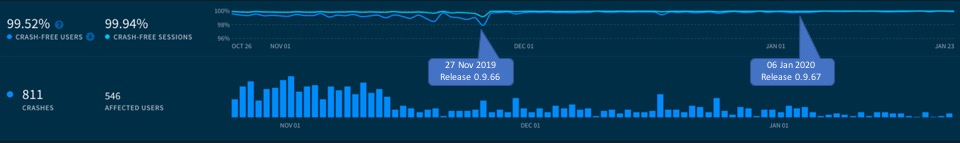
\includegraphics[width=\textwidth]{images/annotated_pocketcode_90_day_fabric_crashlytics_report.jpg}
    \caption{Pocket Code improvements in crash rate, in 90 days}
    %\Description{Pocket Code: When the project team investigated crashes they improved the reliability}
    \label{fig:pocketcode_improvements_in_crash_rate}
\end{figure}

An unacceptably high crash rate for the key Pocket Code Android app were tamed within two releases and 7 weeks by applying the approach described in this thesis. The changes needed to make the improvements were small. Figure \ref{fig:pocketcode_improvements_in_crash_rate} shows the improvement in crash rate as measured by Fabric Crashlytics. When the experiment started the crash rate was nearly four times the maximum threshold recommended by Google in their Android Vitals service and the project team had not been able to address the crash rate despite applying many of the recognised and recommended software development practices over several years~\cite{adamsen2015systematic_catrobat, luhana2018streamlining, ali2019behavior_catrobat, ali2019using_catrobat, hirsch2019approach_catrobat, schranz2019_contributors_impact_on_a_foss_project_quality_catrobat, slany2014tinkering}.

The developers continue to actively use mobile analytics to highlight potential quality issues and address pertinent issues promptly. One of the project teams chose to add an additional analytics tool to both their Android and iOS apps with the objective of improving the teams understanding of broader quality concerns. These quality concerns now also include usability. The team aims to use the data to improve the usability and user experience for their current and future users. They are designing the analytics to retain and protect user privacy, both important and highly relevant concerns.

Mobile Analytics can be incorporated as additional sources of information for development teams in harmony with other sources of information - it is not exclusive or exhaustive.

The analytics tools Google provides to developers of Android apps in Google Play Console have value despite the many flaws my research uncovered in their tools and reports. Some are mentioned in published papers~\cite{harty_google_play_console_insightful_development_using_android_vitals_and_pre_launch_reports, harty_better_android_apps_using_android_vitals, harty_improving_app_quality_despite_flawed_mobile_analytics}, the current known set are in this thesis. The research identified major differences in the reports and analytics provided by two analytics tools from the same company. There were both internal and cross-tool flaws and inconsistencies. Some of these have already been reported to Google in preparation for a full report to be submitted on completion of some ongoing research.

Fully automated pre-launch reports are effective at finding some quality flaws in Android apps at no financial cost and minimal effort by the app developers. These reports are provided by the app store and intended to help developers identify quality issues with their Android apps in order to address these issues so they do not affect end-users.


Google Play uses data collected automatically from users opted-in to provide usage and diagnostics data to Google. The data is collected at a per-device level, which means that one device could potentially report data from several user accounts, conversely for users who use multiple devices some may provide the data while others do not.


\section{Synthesis of a framework for applying mobile analytics effectively}
Bertrand Meyer set an admirable objective for empirical studies - to provide guidance that would help us produce better software and produce software better. 
\begin{quote}
    \emph{``Indeed, this is what we are entitled to expect from empirical studies: guidance. The slogan of empirical software engineering is that software is worthy of study just like geological strata, photons, and lilies-of-the-valley; OK, sure, but we are talking about human artifacts rather than wonders of the natural world, and the idea should be to help us produce better software and produce software better."}~\citep{meyer2018_towards_empirical_answers_to_important_engineering_questions}.
\end{quote}

The experiences and findings gleaned from the various case studies have led to the synthesis of a possible framework for those who wish to use mobile analytics in their software development and software operation practices. This framework emerged from considering various incidents where analytics did, and did not, deliver improvements.

\textit{or?}

The lived experiences of participating in the various case studies, together with the results and insights gleaned from them, led to the synthesis of a potential framework for the successful and effective application of using mobile analytics to improve the reliability of the app. 

These are illustrated in Figure~\ref{fig:using-toc-cpt-using-mobile-analytics-to-improve-mobile-apps}~\footnote{Source of figure, Google Drive file:  \href{https://docs.google.com/document/d/16PaSFRVzg1b2Nykly8qzaTAHtJqtEwgrK754wuek53M/edit}{2021 Applying Theory of Constraints to using Mobile Analytics to improve Mobile Apps} - which needs to be further revised.}. It is based on a diagram known as a conceptual prerequisite tree which is part of Eli Goldratt's Theory of Constraints\footnote{(applying Theory of Constraints, see~\citep{goldratt2017_necessary_but_not_sufficient, lepore1999_deming_and_goldratt, scheinkopf1999_thinking_for_a_change})}. 

Each item is essential in order to \emph{actually} apply mobile analytics in order to improve the quality of mobile apps, \emph{i.e.} they need to be adequately satisfied. Satisfied != perfection. There are other complimentary ways to improve the quality of mobile apps, for instance through designing and implementing automated tests that exercise subsets of the code. Failures reported by mobile analytics are concrete \emph{i.e.} the developers now know the code fails in some circumstances which may motivate the developers to write targeted automated tests. Several of the case studies included developers writing such tests. 

\begin{figure}
    \centering
    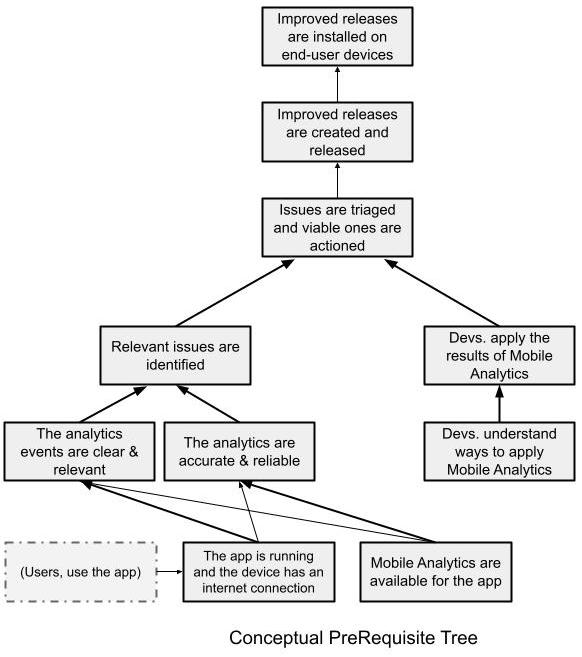
\includegraphics[width=11cm]{images/my/Conceptual_prereq_tree_Applying_Theory_of_Constraints_to_using_Mobile_Analytics_to_improve_Mobile_Apps.jpeg}
    \caption{Conceptual Prerequisites Tree: Using mobile analytics to improve mobile apps}
    \label{fig:using-toc-cpt-using-mobile-analytics-to-improve-mobile-apps}
\end{figure}



% MUST-DO describe the diagram and what each element represents - what each box represents, and each line.
% c.f. \marian{The conceptual prerequisite tree is unclear. She observed it has 2 threads of enquiry; Do the boxes have the same magnitude etc.?}

\textit{I clarified the prerequisites are prerequisites to effective application of mobile analytics. The figure is of a framework either corroborates or revises the approach. It could become an actionable list. Each item identifies a potential points of failure. Or it could be used as a retrospective of the factors I observed. It could be used to reflect on practice. It breaks the topics down.}


%
The underpinnings in terms of being able to improve mobile apps are threefold: 
\begin{enumerate}
    \item Users need to use the app. The app's behaviours will include errors and failures.
    \item The app needs connectivity together with at least one form of mobile analytics.
    \item Developers need to understand the outputs of mobile analytics and address pertinent issues in future releases of the app.
\end{enumerate}

An expanded list of the prerequisites illustrated in Figure~\ref{fig:using-toc-cpt-using-mobile-analytics-to-improve-mobile-apps} is as follows (roughly in descending order. Analytics data from previous releases is used to help improve \emph{future} releases.

\Prerequisite{Essential prerequisites to improve the reliability of apps using mobile analytics}
{\small
\begin{enumerate}
    \itemsep0em
    \item Users use the app
    \item Improved releases are in-use on end-user devices
    \item Improved releases are installed on end-user devices
    \item Improved releases are created and released
    \item Analytics logging refined to capture relevant information
    \item Issues are triaged and viable ones actioned
    \item Devs have adequate, timely access to mobile analytics outputs
    \item Devs apply the results of mobile analytics outputs
    \item Devs understand ways to apply mobile analytics
    \item Relevant issues are identified and analysed
    \item The analytics service is accurate and reliable
    \item The analytics events are clear and relevant
    \item Volumes of data do not overwhelm system or devs
    \item The app is running and the device has an internet connection
    \item Mobile analytics are available for the app
    \captionof{prerequisites}{Prerequisites to improve the reliability of apps using mobile analytics}
    \label{prerequisites-essential}
\end{enumerate}
}
Note: The stack traces reported in Google's Android Vitals are not always sufficient to identify the failure. One example where it's insufficient is \href{insight-expo-stack-trace-not-sufficient-to-identify-the-failure}{GitHub Expo Issue 5839}.

\Prerequisite{Additional, desirable prerequisites}
In addition to the essential set of prerequisites, in ~\ref{prerequisites-essential}, the following are also highly desirable:
{\small
\begin{enumerate} %[i]
    \itemsep0em
    \item Ecosystem is adequately and acceptably secure
    \item System is performant
    \item System is unbiased
    \item Internally and externally verifiable system and service
    \item Users have practical controls on the data processed
    \item Available data sufficiently representative to apply to the population
    \item Current and historical data and reports seamlessly available to development team
    \captionof{prerequisites}{Additional, desirable prerequisites when using mobile analytics}
    \label{prerequisites-desirable}
\end{enumerate}
}


\subsection{Guidance for researchers}

\subsection{Guidance for practitioners}
